Este capítulo detalha o estado atual de desenvolvimento do protótipo físico do robô de serviço proposto neste trabalho. A construção deste protótipo corresponde à materialização do artefato definido na metodologia, especificamente na Etapa 2 da \textit{Design Science Research} (DSR), voltada ao desenvolvimento e integração da solução. O foco desta etapa concentrou-se em obter uma plataforma física funcional, capaz de integrar atuadores, sensores, comunicação serial, ROS 2 e aquisição de dados RGB-D para posterior execução do pipeline de SLAM visual embarcado.

O propósito central do protótipo físico é mitigar os riscos do projeto ao assegurar uma base realista e operacional para os experimentos de mapeamento. O artefato deve viabilizar a avaliação do RTAB-Map em hardware restrito, a observação da estabilidade dos tópicos e transformações, e a análise de ajustes de odometria e fusão sensorial. Assim, ainda que um sistema completo de navegação autônoma não tenha sido alcançado nesta fase, consolidou-se uma infraestrutura de hardware e software suficiente para a realização dos testes de SLAM embarcado planejados.

\section{Objetivos do Protótipo Físico nesta Etapa}

Nesta fase de desenvolvimento, os objetivos do protótipo físico foram deliberadamente definidos de forma incremental. O escopo não abrangeu a implementação definitiva de um sistema de navegação autônoma completo, mas sim a validação dos elementos fundamentais que sustentam a arquitetura proposta. Entre os objetivos específicos desta etapa, destacam-se:

\begin{itemize}
    \item Implementação do chassi com seus componentes principais, incluindo os motores do chassi reaproveitado, o microcontrolador responsável pela interface com hardware (camada de controle de atuadores), a unidade de processamento de alto nível (Raspberry) e os sensores (Kinect e IMU).
    \item Assegurar a movimentação confiável do robô, permitindo a validação do circuito de potência, da ponte H e do \textit{firmware} responsável pelo controle dos motores;
    \item Viabilizar a leitura contínua dos dados da unidade de medição inercial (IMU) e estabelecer o fluxo de publicação desses dados no ambiente \textit{Robot Operating System} (ROS 2);
    \item Realizar testes preliminares de integração da câmera RGB-D com o ROS 2, preparando a infraestrutura para a execução do RTAB-Map;
    \item Validar a organização dos tópicos, transformações e fluxos de dados necessários para avaliação do SLAM visual embarcado.
\end{itemize}

Dessa forma, ainda que a navegação autônoma completa não tenha sido integrada, consolidou-se a infraestrutura necessária para executar e avaliar o mapeamento visual no próprio robô físico.

\section{Arquitetura Física do Protótipo}

Do ponto de vista físico, o protótipo consiste em um robô móvel que integra três subsistemas principais interconectados:  a unidade computacional (Raspberry Pi), o sistema de percepção (câmera RGB-D e IMU) e a camada de interface com hardware (microcontrolador Arduino Nano, drivers e atuadores). A arquitetura foi projetada para validar a comunicação e o fluxo de dados entre esses componentes, garantindo a infraestrutura necessária para a execução dos algoritmos de navegação. A Figura \ref{fig:diagrama_ligacao} ilustra o diagrama de ligação em alto nível entre estes componentes, evidenciando a topologia de comunicação e alimentação.

\begin{figure}[h!]
    \centering
    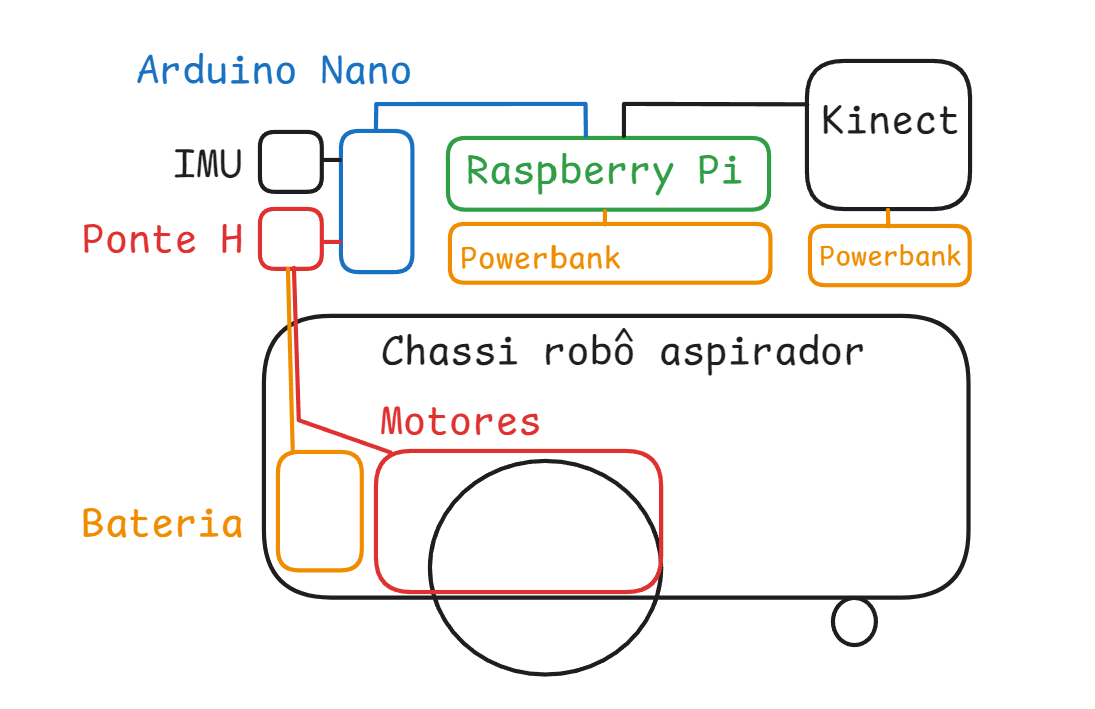
\includegraphics[width=0.8\textwidth]{figuras/DiagramLigacao.png}
    \caption{Diagrama de ligação dos componentes do protótipo físico em alto nível.}
    \label{fig:diagrama_ligacao}
    Elaborado pelo autor (2025).
\end{figure}

A organização do sistema segue uma abordagem em camadas. Na base, encontra-se o chassi mecânico com o sistema de tração e a fonte de energia primária. Acima, a camada de hardware embarcado gerencia os sinais elétricos, a leitura de sensores e a comunicação serial. Na camada superior, a unidade de processamento executa o sistema operacional e o \textit{middleware} robótico, centralizando a lógica de integração, percepção e mapeamento.

\subsection{Plataforma Mecânica Reaproveitada}

A base mecânica do protótipo foi obtida a partir do reaproveitamento de um chassi de robô aspirador comercial, selecionado por sua robustez e adequação para ambientes internos. O sistema de locomoção adota a cinemática de tração diferencial, caracterizada pelo acionamento de duas rodas laterais independentes, cada uma acoplada a seu respectivo motor de corrente contínua, auxiliadas por uma roda de apoio frontal para garantir o equilíbrio estático e dinâmico. A Figura \ref{fig:robo_original} apresenta o chassi utilizado antes das adaptações estruturais.

\begin{figure}[h!]
    \centering
    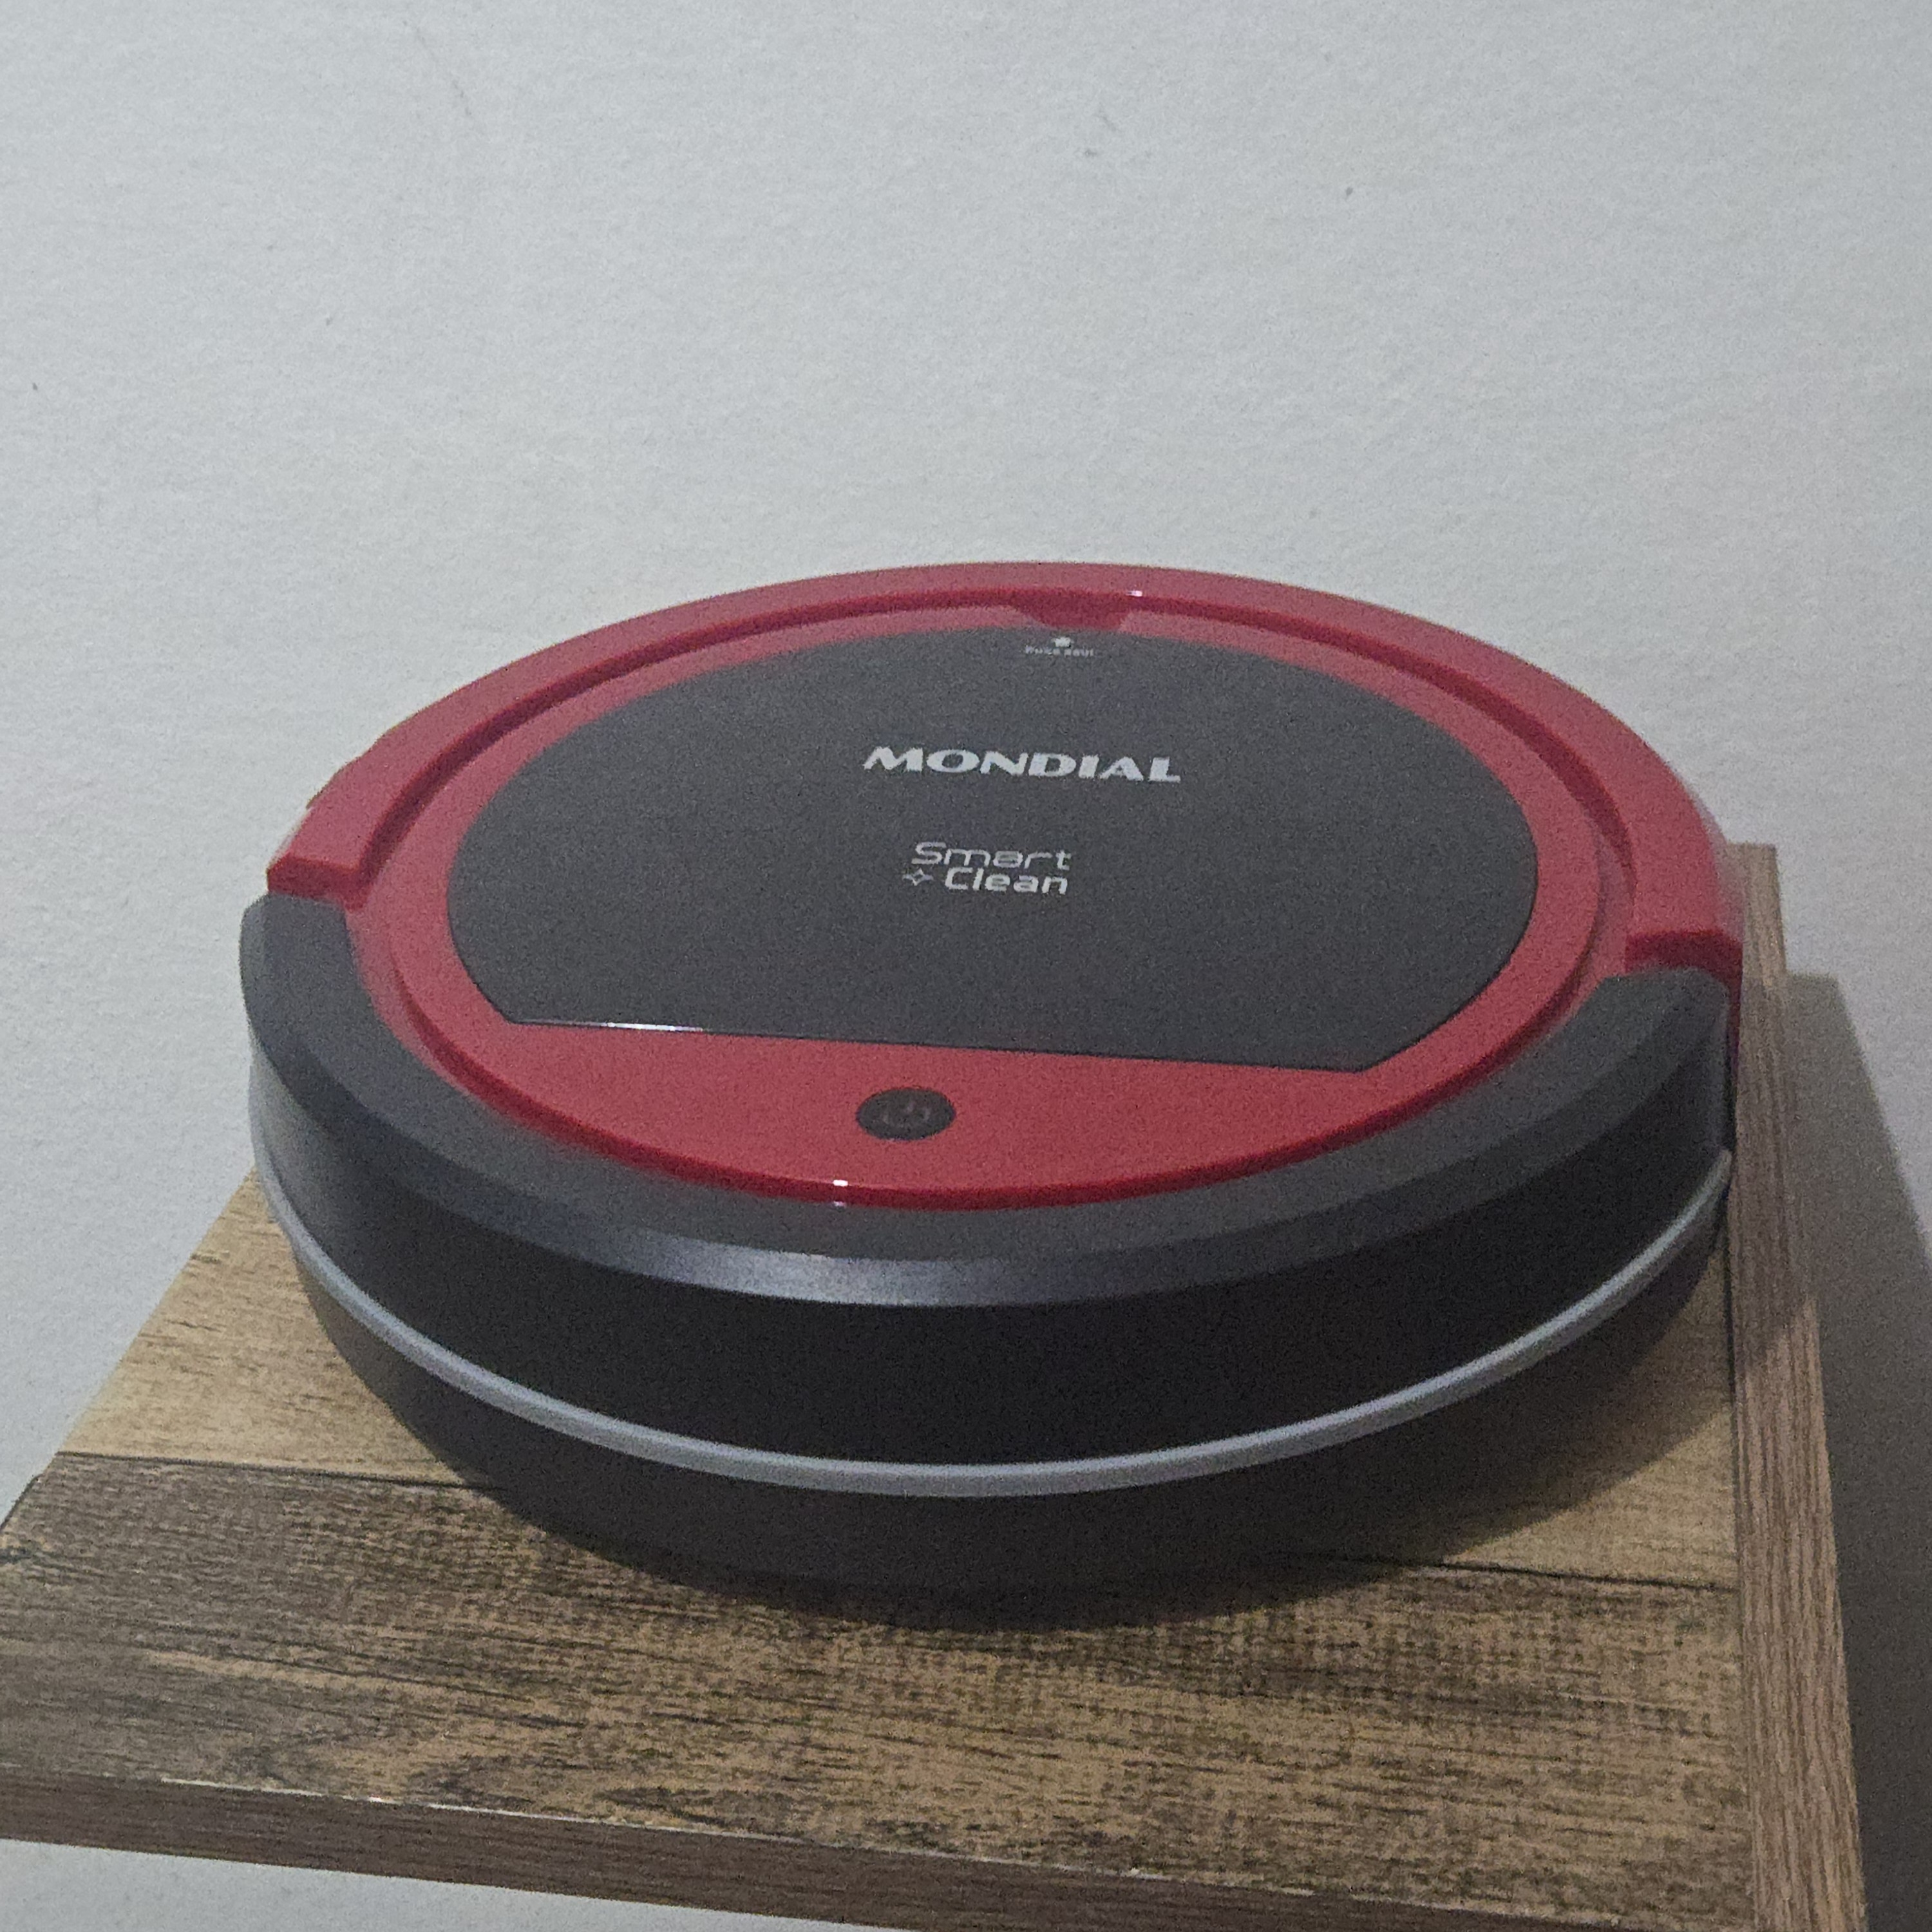
\includegraphics[width=0.6\textwidth]{figuras/chassi.jpg}
    \caption{Chassi do robô aspirador utilizado como base mecânica.}
    \label{fig:robo_original}
    Foto tirada pelo autor (2025).
\end{figure}

A escolha por reaproveitar esta plataforma justifica-se pela redução de custos e tempo de desenvolvimento, visto que os motores e o sistema de redução já se encontram integrados e dimensionados para a carga de trabalho doméstica. Para adaptar a plataforma aos requisitos da pesquisa, os circuitos proprietários originais foram removidos. A superfície superior do chassi foi utilizada para a fixação dos novos componentes eletrônicos, incluindo o computador de placa única, o microcontrolador, os drivers de potência e a câmera RGB-D, mantendo a eletrônica acessível para manutenção e ajustes durante os experimentos. A Figura \ref{fig:prototipo_final} exibe o protótipo com a integração física dos componentes concluída.

\begin{figure}[h!]
    \centering
    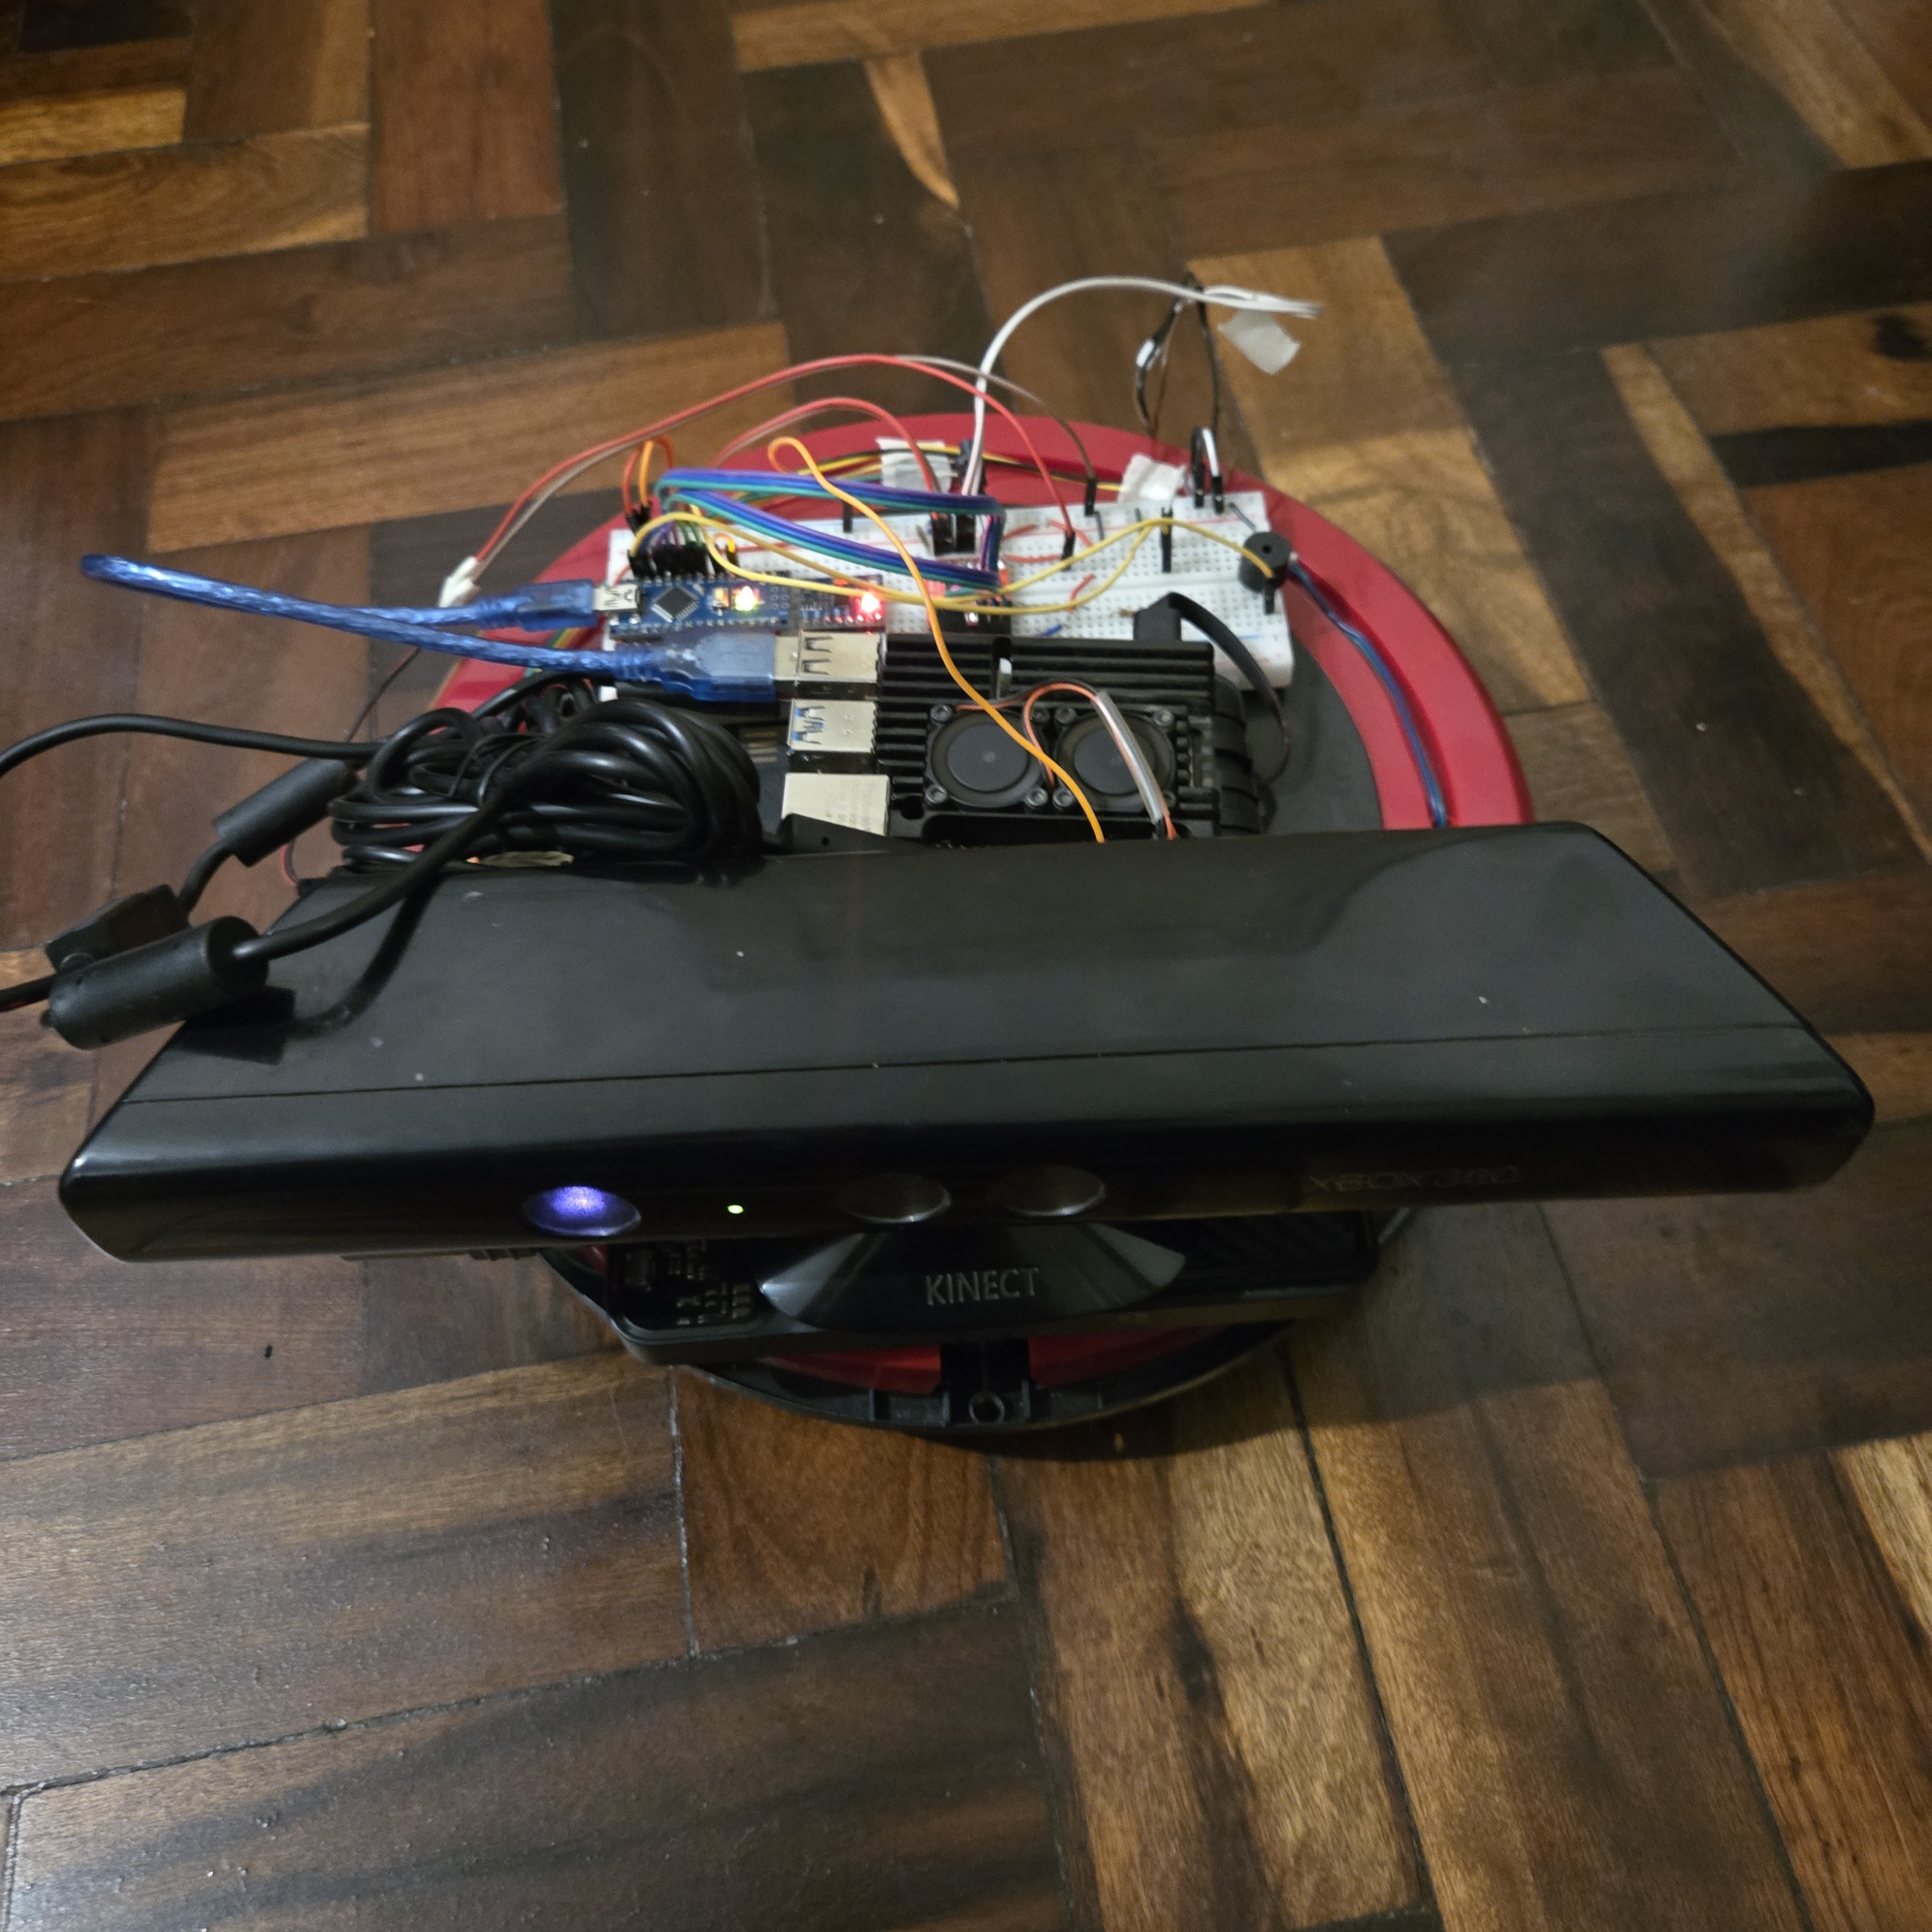
\includegraphics[width=0.7\textwidth]{figuras/prototipo1.jpg}
    \caption{Protótipo físico com integração dos componentes de processamento e percepção.}
    \label{fig:prototipo_final}
    Foto tirada pelo autor (2025).
\end{figure}


\subsection{Microcontrolador de Controle e Atuadores}

O controle dos atuadores e a interface de hardware de baixo nível são gerenciados por um microcontrolador Arduino Nano \cite{arduino2024arduinonano, atmel2012atmega328p8bit}, que atua como intermediário entre a unidade de processamento de alto nível e os atuadores físicos. Este dispositivo executa um \textit{firmware} dedicado ao recebimento de comandos de velocidade linear e angular via interface serial, convertendo-os em sinais de modulação por largura de pulso (PWM) e direção. O acionamento dos motores de corrente contínua é realizado por uma ponte H modelo TB6612FNG \cite{microsemi2015tb6612fngdriver}, cuja operação exige a configuração específica do pino de \textit{standby} (STBY) em nível lógico alto para a habilitação correta das saídas de potência.

No que tange à percepção inercial, o microcontrolador realiza a leitura periódica de um sensor MPU-6050 \cite{invensense2013mpu6050} via barramento I\textsuperscript{2}C \cite{nxp2021i2cbus}. Os dados brutos de aceleração e velocidade angular são adquiridos e encapsulados em mensagens compactas, enviadas de volta ao computador de placa única através do mesmo enlace serial utilizado para o controle. Esse fluxo de dados bidirecional segue um protocolo definido para garantir a integridade das informações e a execução de tarefas em tempo real, fundamentais para a estabilidade da navegação.

O sistema de alimentação foi segmentado para minimizar interferências e garantir a robustez do circuito. O estágio de potência, composto pela ponte H e pelos motores de tração, é energizado por uma bateria de íons de lítio de três células (3S), gerenciada por um sistema de proteção BMS (\textit{Battery Management System}) \cite{texas_instruments2022bq78_bms}. Em contrapartida, a lógica de controle do microcontrolador é alimentada diretamente pela conexão USB estabelecida com a unidade de processamento de alto nível (Raspberry Pi), isolando o processamento dos ruídos elétricos gerados pela carga indutiva dos motores.

\subsection{Unidade de Processamento de Alto Nível}

A unidade de processamento de alto nível é constituída por um computador de placa única (\textit{Single Board Computer} - SBC) Raspberry Pi 4 Model B \cite{raspberrypi2019raspberrypi}, equipado com 8 GB de memória RAM \cite{broadcom2021bcm2711arm}. Essa unidade é responsável por orquestrar os diferentes nós de software, integrar dados de sensores, enviar comandos ao microcontrolador e executar os componentes centrais do pipeline embarcado.

Quanto ao software de base, optou-se pelo sistema operacional Ubuntu 24.04 LTS (\textit{Noble Numbat} \cite{canonical2024ubuntu2404}), arquitetura \textit{aarch64}, instalado em modo servidor (\textit{headless}). A ausência de interface gráfica de usuário (GUI) libera recursos críticos de CPU e memória para os processos robóticos. Sobre o sistema operacional, foi configurado o ambiente ROS 2 na distribuição Jazzy Jalisco \cite{openrobotics2024jazzy}, responsável pela orquestração dos nós, gerenciamento de mensagens e comunicação entre processos.

No contexto deste protótipo físico, a unidade de processamento hospeda os seguintes pacotes e funcionalidades essenciais:

\begin{itemize}
    \item \textbf{Interface de Hardware (Drivers):} Execução dos nós responsáveis pela comunicação direta com a câmera RGB-D (via biblioteca \textit{libfreenect} \cite{openkinect2010libfreenect}) e com o microcontrolador (via protocolo serial customizado);
    \item \textbf{Teleoperação:} Pacotes para interfaceamento com dispositivos de entrada (\textit{joystick}), convertendo interações físicas do operador em comandos de velocidade (\textit{Twist}) padronizados;
    \item \textbf{Infraestrutura de Comunicação:} Configuração do \textit{middleware} Eclipse Cyclone DDS \cite{eclipse2021eclipsecyclonedds} para garantir a comunicação eficiente entre os nós do sistema;
    \item \textbf{Pré-processamento e SLAM:} Nós preliminares de visualização e mapeamento, configurados para receber os fluxos de dados da câmera, da IMU e da odometria, preparando o sistema para a execução do RTAB-Map.
\end{itemize}

O dispositivo de controle manual (\textit{joystick}) utilizado nos testes é reconhecido pelo sistema operacional como um dispositivo de entrada padrão. Sua integração ao ROS 2 ocorre por meio de nós específicos que leem o estado dos eixos e botões, publicando-os em tópicos de comando. Essa configuração fornece a base computacional necessária para a operação do robô, permitindo a integração lógica dos componentes que será detalhada na seção a seguir.

\section{Integração de Software e Sensores}

A integração lógica do protótipo é orquestrada pelo \textit{framework} ROS 2, que organiza o sistema em um grafo de nós comunicantes. A arquitetura de software foi estruturada para garantir o fluxo eficiente de dados entre a camada de controle (Arduino), os sensores de percepção e a unidade de processamento central (Raspberry Pi). Utilizou-se o \textit{middleware} Eclipse Cyclone DDS para o transporte de mensagens, visando minimizar a latência na comunicação entre processos e na rede local.

\subsection{Controle e Sensoriamento Inercial}

A comunicação entre a unidade de processamento de alto nível e o hardware de atuação é mediada por um nó de interface serial desenvolvido em Python. A Figura \ref{fig:script_serial} apresenta a execução deste nó no Raspberry Pi. O terminal exibe o estabelecimento da conexão com a porta \texttt{/dev/ttyUSB0} e o fluxo bidirecional de dados: o envio de comandos de velocidade (linear e angular) para o microcontrolador e o recebimento de confirmações de execução.

\begin{figure}[H]
    \centering
    \caption{Execução do \textit{script} de interface serial validando a comunicação com o microcontrolador.}
    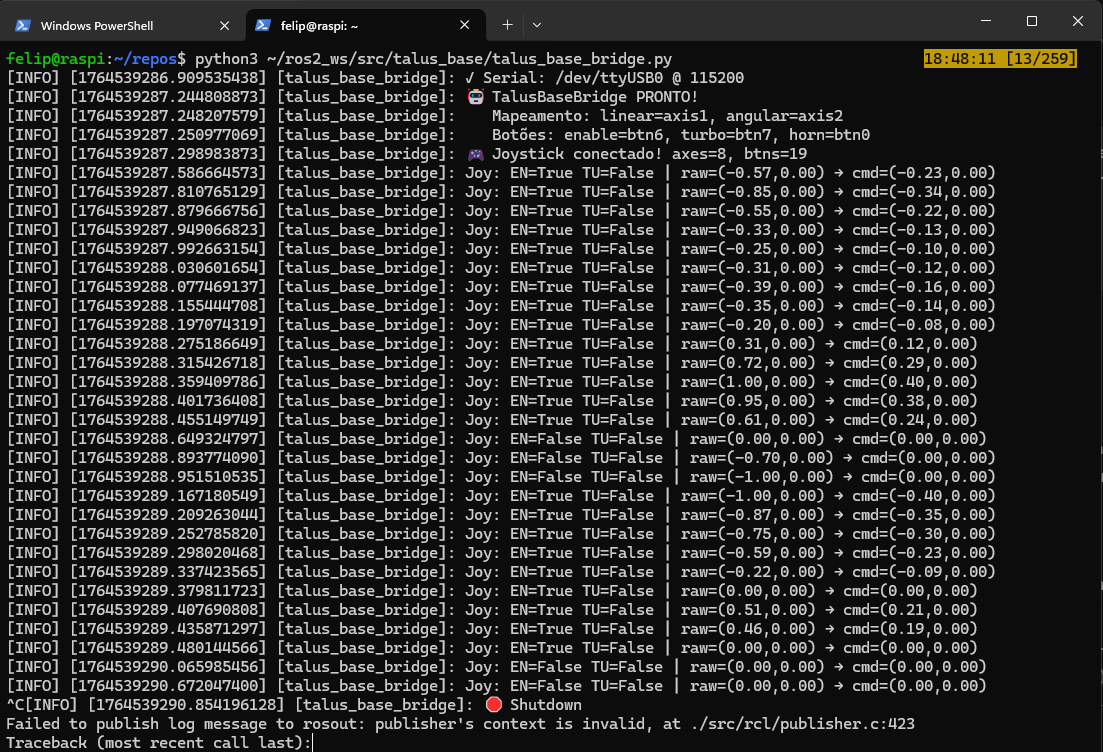
\includegraphics[width=0.85\textwidth]{figuras/scriptPythonArduino.png}
    \label{fig:script_serial}
    \fonte{Autor (2025).}
\end{figure}

No sentido inverso, o sistema realiza a aquisição dos dados da unidade de medição inercial (IMU). O microcontrolador lê os registros do sensor MPU-6050 via barramento I\textsuperscript{2}C e os transmite via serial. O nó de interface no ROS 2 decodifica esses pacotes e publica os dados no tópico padronizado \texttt{/imu/data}. A Figura \ref{fig:topicos_imu} comprova a eficácia desta integração: o terminal superior demonstra que os dados estão sendo publicados a uma frequência estável de aproximadamente 49 Hz, taxa ideal para algoritmos de fusão sensorial, enquanto o terminal inferior exibe a estrutura das mensagens contendo vetores de orientação e velocidade angular.

\begin{figure}[H]
    \centering
    \caption{Validação da frequência (49 Hz) e dos dados do tópico de IMU.}
    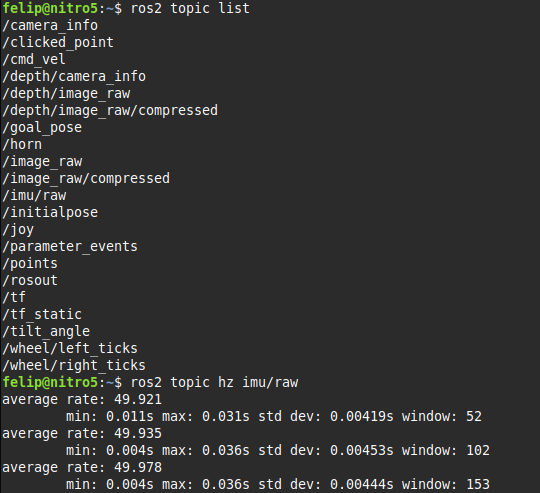
\includegraphics[width=0.85\textwidth]{figuras/ROSarduinoTopicsIMU.png}
    \label{fig:topicos_imu}
    \fonte{Autor (2025).}
\end{figure}

\subsection{Integração do Sensor Visual RGB-D}

A integração da câmera RGB-D (Kinect v1) exigiu a configuração de regras de permissão (\textit{udev}) no Linux embarcado e a compilação da biblioteca \textit{libfreenect}. A inicialização bem-sucedida do driver é apresentada na Figura \ref{fig:comando_kinect}, onde o sistema reconhece o dispositivo USB e inicia a publicação dos tópicos de imagem e profundidade sem erros de alocação de recurso.

\begin{figure}[H]
    \centering
    \caption{Inicialização do driver da câmera RGB-D no ambiente ROS 2.}
    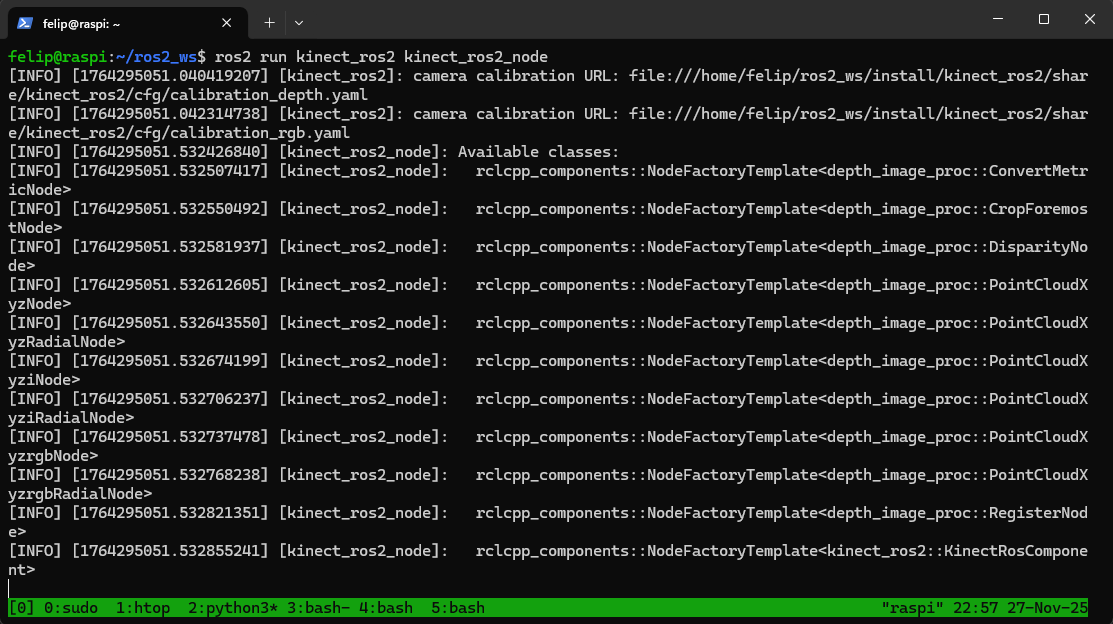
\includegraphics[width=0.85\textwidth]{figuras/comandoROSkinect.png}
    \label{fig:comando_kinect}
    \fonte{Autor (2025).}
\end{figure}

Um dos principais riscos do uso de vSLAM em SBCs (\textit{Single Board Computers}) é a sobrecarga da CPU durante a aquisição de imagens. Para verificar esse gargalo, monitorou-se a taxa de quadros localmente no Raspberry Pi. Conforme demonstra a Figura \ref{fig:hz_local}, o sistema manteve uma taxa estável de aproximadamente 30.03 Hz (limite físico do sensor), comprovando que o hardware selecionado possui capacidade de processamento suficiente para a etapa de aquisição de dados sem perda de \textit{frames}.

\begin{figure}[H]
    \centering
    \caption{Monitoramento da taxa de quadros (Hz) do sensor visual executado localmente no Raspberry Pi.}
    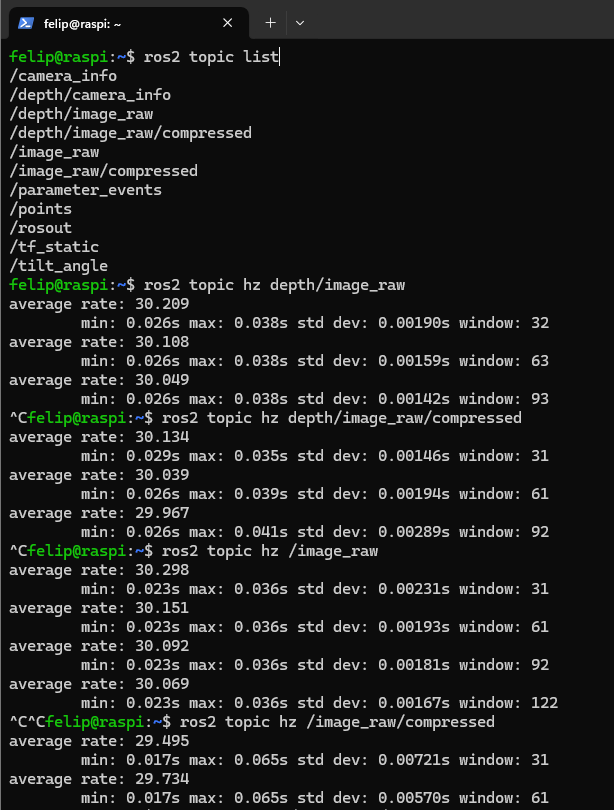
\includegraphics[width=0.7\textwidth]{figuras/ROSkinectHZraspi.png}
    \label{fig:hz_local}
    \fonte{Autor (2025).}
\end{figure}

Após a inicialização de todos os drivers e interfaces, foi possível validar a arquitetura completa de tópicos do sistema. A Figura \ref{fig:lista_topicos} apresenta a listagem dos canais de comunicação ativos, evidenciando a presença simultânea dos tópicos de percepção visual (\texttt{/depth/...}, \texttt{/image\_raw}), inercial (\texttt{/imu/raw}), odometria (\texttt{/wheel/...}) e controle (\texttt{/cmd\_vel}, \texttt{/joy}), confirmando a integração bem-sucedida de todos os subsistemas.

\begin{figure}[H]
    \centering
    \caption{Listagem dos tópicos ativos no ROS 2 evidenciando a integração de todos os sensores e atuadores.}
    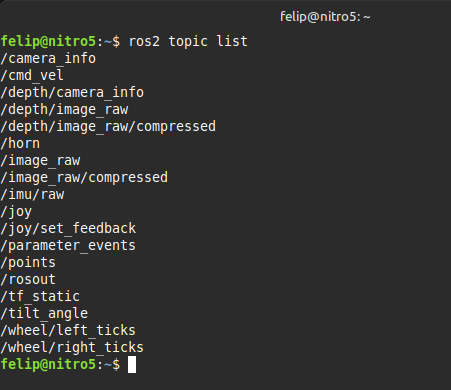
\includegraphics[width=0.6\textwidth]{figuras/rosTopicListNitro5.png}
    \label{fig:lista_topicos}
    \fonte{Autor (2025).}
\end{figure}


\section{Validação Experimental Preliminar}

Com a integração física e lógica concluída, foram realizados experimentos funcionais para validar a operabilidade do protótipo. Estes testes tiveram caráter exploratório, visando assegurar que a infraestrutura de \textit{hardware}, a pilha de \textit{software} e a comunicação em rede atendem aos requisitos mínimos para os experimentos de SLAM visual previstos na próxima fase da pesquisa.

\subsection{Validação da Comunicação e Observabilidade}

A arquitetura proposta depende de comunicação estável entre os nós do ROS 2 e de observabilidade suficiente para inspecionar os dados gerados pelo robô durante os testes. Para validar este requisito, o protótipo foi conectado à rede local via Wi-Fi (5 GHz), recebendo endereçamento estático para facilitar a descoberta de nós pelo \textit{middleware} Cyclone DDS e permitir o monitoramento externo dos tópicos.

A estabilidade da transmissão de dados foi verificada monitorando a frequência de recebimento na estação de trabalho utilizada para inspeção. A Figura \ref{fig:hz_remoto} exibe o terminal recebendo o tópico de profundidade a uma taxa média de 30.04 Hz, compatível com a taxa de geração no robô. Isso confirma que a infraestrutura de rede permite visualizar e registrar os dados do sistema durante os ensaios, sem transformar o processamento remoto em eixo de avaliação do trabalho.

\begin{figure}[H]
    \centering
    \caption{Estabilidade da recepção de dados visuais na estação remota (30 Hz via Wi-Fi).}
    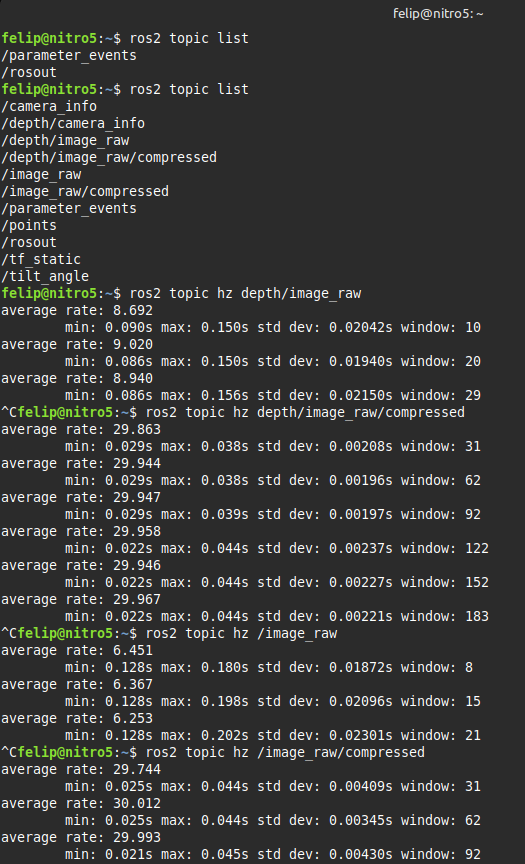
\includegraphics[width=0.7\textwidth]{figuras/ROSkinectHZnitro.png}
    \label{fig:hz_remoto}
    \fonte{Autor (2025).}
\end{figure}

Além da frequência, analisou-se a largura de banda exigida para a transmissão dos dados visuais durante a observação externa. Conforme apresentado na Figura \ref{fig:bandwidth_rede}, a transmissão das imagens brutas (\textit{raw}) de profundidade e RGB consome, respectivamente, cerca de 5.55 MB/s e 6.75 MB/s. Este volume de dados justifica a escolha da frequência de 5 GHz para a rede sem fio e evidencia a necessidade de cautela ao registrar ou visualizar tópicos de imagem durante os experimentos.

\begin{figure}[H]
    \centering
    \caption{Análise de largura de banda consumida pelos tópicos de imagem na rede local.}
    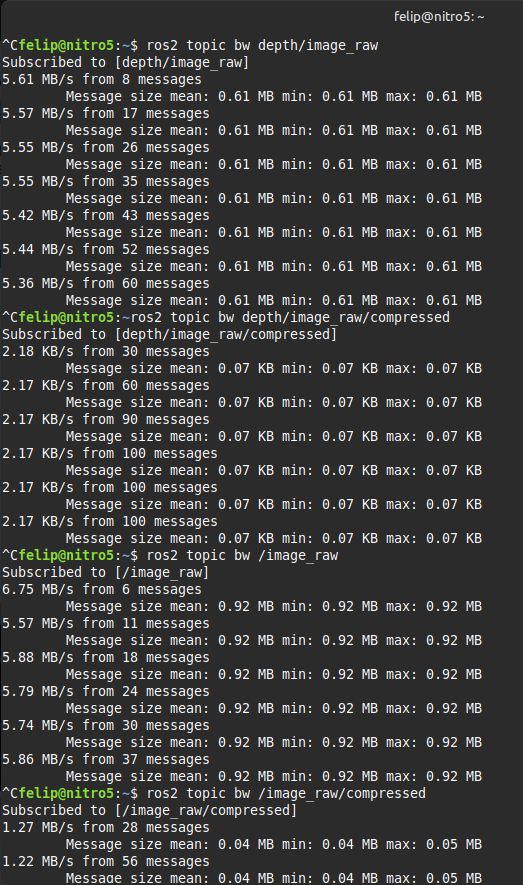
\includegraphics[width=0.7\textwidth]{figuras/ROSkinectBWnitro.png}
    \label{fig:bandwidth_rede}
    \fonte{Autor (2025).}
\end{figure}

\subsection{Teleoperação e Resposta Dinâmica}

A validação do sistema de locomoção foi realizada por meio de teleoperação assistida. Um nó de interface foi configurado para traduzir as entradas de um \textit{joystick} em comandos de velocidade linear e angular. Antes de atuar nos motores, verificou-se a integridade dos dados de entrada. A Figura \ref{fig:joy_echo} demonstra a captura dos vetores dos eixos analógicos (\textit{axes}) e o estado dos botões digitais (\textit{buttons}) do controle, confirmando que o nó de teleoperação interpreta corretamente as ações do usuário.

\begin{figure}[H]
    \centering
    \caption{Verificação dos dados de entrada do \textit{joystick} no tópico \texttt{/joy}.}
    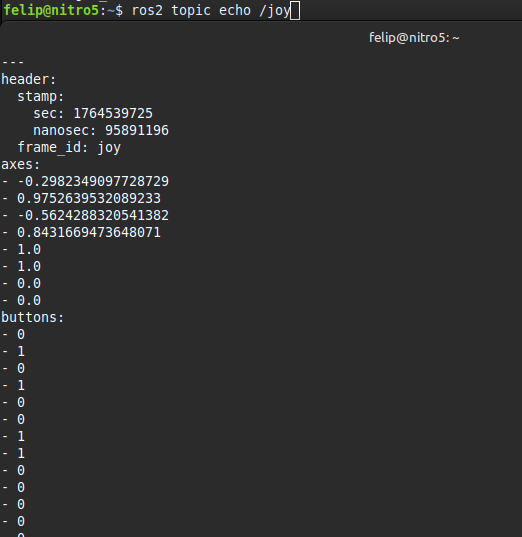
\includegraphics[width=0.6\textwidth]{figuras/rosJoyEchoNitro5.png}
    \label{fig:joy_echo}
    \fonte{Autor (2025).}
\end{figure}

Durante os ensaios de movimentação em ambiente interno, verificou-se:
\begin{itemize}
    \item \textbf{Resposta dos Atuadores:} Os motores responderam de forma proporcional aos comandos, validando a lógica de PWM e o dimensionamento da ponte H;
    \item \textbf{Estabilidade Elétrica:} Não foram observadas quedas de tensão ou reinicializações do microcontrolador durante picos de corrente (partida dos motores), validando o isolamento da alimentação lógica e de potência.
\end{itemize}

\subsection{Aquisição de Dados de Percepção}

Paralelamente à movimentação, avaliou-se a qualidade dos dados de percepção. As séries temporais da IMU foram capturadas durante rotações e acelerações, apresentando comportamento consistente com a dinâmica do robô.

A Figura \ref{fig:rviz_interface} apresenta a interface da estação de trabalho recebendo os dados do robô em tempo real, onde é possível observar o painel de configuração dos tópicos e a janela de visualização da câmera.

\begin{figure}[H]
    \centering
    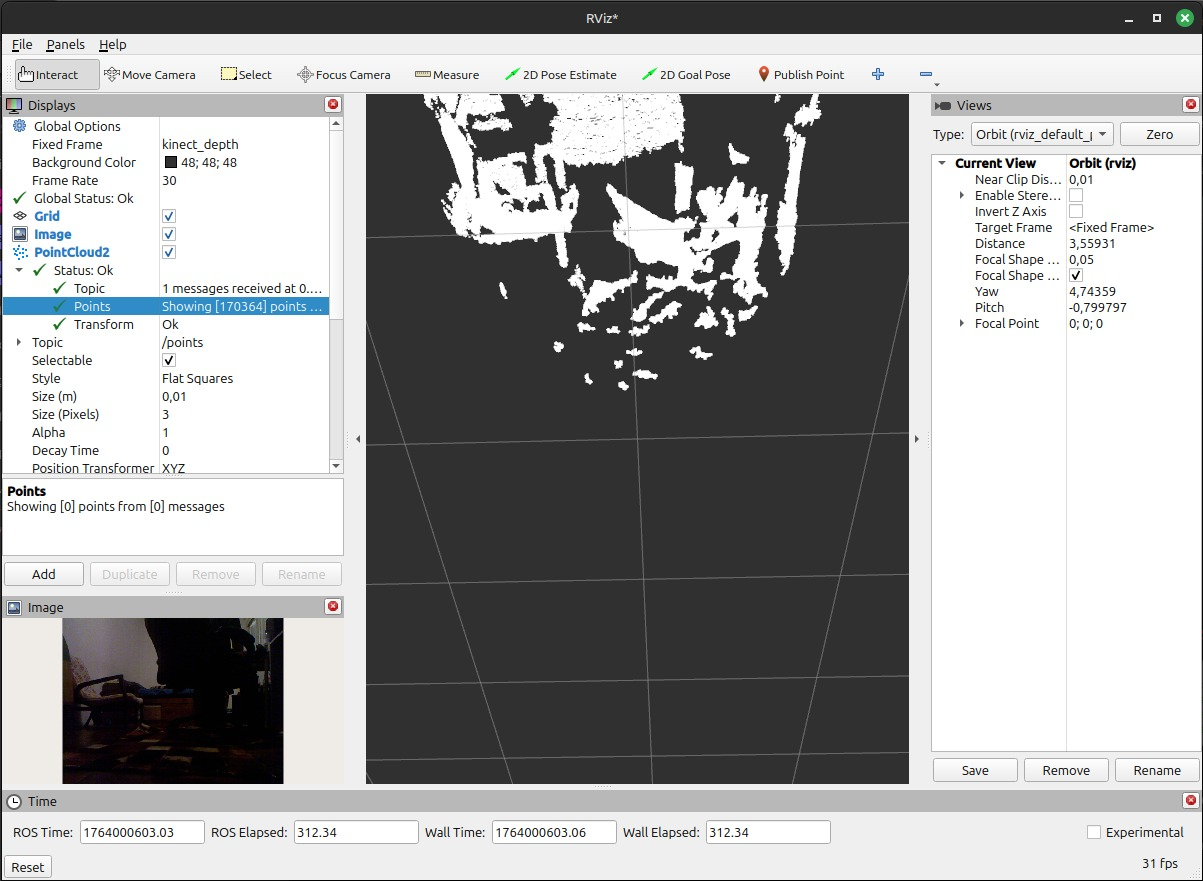
\includegraphics[width=0.9\textwidth]{figuras/rviz2.jpg}
    \caption{Interface de visualização RViz na estação remota recebendo dados do robô.}
    \label{fig:rviz_interface}
    \fonte{Autor (2025).}
\end{figure}

A qualidade da reconstrução 3D do ambiente pode ser observada na Figura \ref{fig:nuvem_pontos}, que exibe a nuvem de pontos gerada a partir do mapa de profundidade. A densidade e a coerência geométrica dos pontos demonstram que o sensor está calibrado e posicionado adequadamente para as tarefas de mapeamento. A captura dos dados brutos (\textit{raw data}) mostrou-se robusta, fornecendo a base necessária para a execução do RTAB-Map no protótipo físico.

\begin{figure}[H]
    \centering
    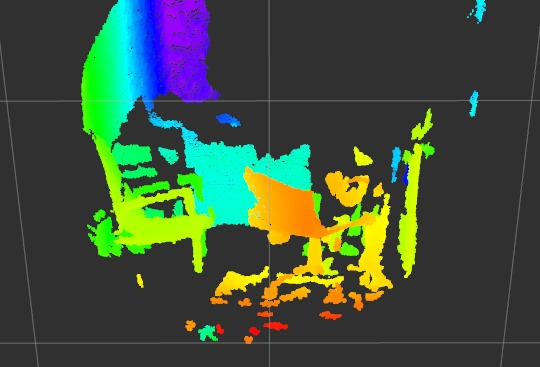
\includegraphics[width=0.7\textwidth]{figuras/pointCloud.jpg}
    \caption{Detalhe da nuvem de pontos 3D capturada em ambiente interno.}
    \label{fig:nuvem_pontos}
    \fonte{Autor (2025).}
\end{figure}

\section{Limitações Atuais e Encaminhamentos Futuros}

O desenvolvimento do protótipo físico atingiu o objetivo de estabelecer um MVP (\textit{Minimum Viable Product}) funcional de robótica móvel. No entanto, como previsto na metodologia incremental, o sistema encontra-se em estágio intermediário.

As principais limitações identificadas nesta etapa, que definem o escopo do Trabalho de Conclusão de Curso II (TCC II), incluem:
\begin{itemize}
    \item \textbf{SLAM Embarcado:} A execução estável de algoritmos de mapeamento visual no Raspberry Pi requer otimizações de software e ajustes finos de parâmetros que não foram concluídos nesta fase;
    \item \textbf{Autonomia de Navegação:} A pilha de navegação (\textit{Nav2}) para planejamento de trajetória e desvio de obstáculos ainda não foi integrada ao controle de baixo nível, permanecendo como continuidade futura após a estabilização do mapeamento e da localização;
    \item \textbf{Evidências Experimentais:} A consolidação final das métricas de SLAM, incluindo perda de pose, estabilidade do mapa e comparação antes/depois de ajustes de odometria, ainda depende da conclusão dos ensaios controlados.
\end{itemize}

Apesar destas lacunas, a contribuição desta etapa é significativa: consolidou-se uma plataforma de baixo custo com \textit{drivers} funcionais, comunicação entre componentes validada, sensores operacionais e integração de hardware suficiente para os experimentos de SLAM visual. Esta base reduz substancialmente o risco técnico do projeto e habilita a execução dos testes sistemáticos propostos na metodologia.
